\chapter{Solución}

El rediseño de software llevado a cabo mantiene el diseño original del framework, agregándole nuevas funcionalidades para brindar
interactividad entre servidor y cliente de manera que \rc{} puede acoplarse a él. Ésto permite que aplicaciones que corrían sobre \fud{}
original sigan haciéndolo, con la opción a usar las nuevas características que serán presentadas a continuación.

\section{Nuevas funcionalidades}

Concretamente, las funcionalidades requeridas por \rc{} que forman parte del rediseño del framework son:
\begin{itemize}
    \item   envío de mensajes de cliente a servidor, y
    \item   pedido y reserva de clientes.
\end{itemize}
A continuación veremos, en detalle, cada uno de ellos.

\subsection{Envío de mensajes}

La importancia de este punto es la libertad que el cliente obtiene pudiendo enviar mensajes cuando desee y, así, el servidor por ejemplo
poder ir reduciendo resultados o conocer del estado de cada cliente, sin que éstos dejen de procesar su trabajo asignado.

Ya que en \fud{} original el cliente sólo enviaba un resultado al fin del procesamiento, ésto significaba que el cliente había terminado de
ejecutar su tarea. Con la implementación de esta nueva funcionalidad, se debió añadir un paquete que informa que una unidad de trabajo ha
finalizado y por ende, el cliente que lo envió es libre nuevamente.

A continuación se dan las responsabilidades que deben atender tanto el cliente como el servidor:
\begin{itemize}
    \item   \underline{Cliente}\\Permitir que el cliente envíe mensajes en cualquier momento y la cantidad de veces que desee, sin necesidad
            de cortar su ejecución. Cuando termine de ejecutar su unidad de trabajo, debe enviar el paquete de finalización.
    \item   \underline{Servidor}\\Permitir que el servidor reciba cualquier cantidad de mensajes de un cliente en particular, y recién
            marcarlo como un cliente ocioso y a su trabajo asigando como finalizado cuando éste le envíe un paquete de finalización.
\end{itemize}


\subsection{Pedido y reserva de clientes}

Un cliente podrá saber sobre la disponibilidad de clientes ociosos, y más aún podrá reservar una cantidad para su uso. El uso de esta
funcionalidad trae aparejado una mayor responsabilidad para los clientes, ya que su utilización en demasía sobrecarga al servidor de
consultas, con ello disminuye demasiado la cantidad de clientes libres del framework y, por lo tanto, la performance total del proyecto
podría decaer drásticamente.

Las responsabilidades de los dos actores de esta comunicación son:
\begin{itemize}
    \item   \underline{Cliente}\\Otorgar la posibilidad de que el cliente pregunte al servidor sobre la disponibilidad de clientes libres
            y espere una eventual respuesta del servidor. Será el número de clientes ociosos que el servidor desee designar en un momento
            dado, quedando así reservados a merced del cliente que realizó la pregunta.
    \item   \underline{Servidor}\\Debe recibir la consulta por clientes libres, calcular el número de clientes ociosos que desee enviar
            como respuesta, y en caso de que el número fuera positivo, reservará esa cantidad de clientes no pudiendo ser usados durante
            un tiempo estipulado.
\end{itemize}

Este \textit{feedback} entre cliente y servidor le permite a \rc{} redistribuir los functores hijos de un cliente a otros clientes ociosos
con el fin de balancear la carga de trabajo, y así lograr un alto rendimiento en la ejecución de aplicaciones. En otras palabras, permite
generar unidades de trabajo a demanda, asegurándose que existen clientes libres para procesar estas tareas.

 
\section{Diseño}
\label{redesign_design}

Como se dijo anteriormente, se mantuvo el diseño original del framework, no hubo cambios radicales, salvo la inclusión de dos nuevas clases
y la modificación de, alrededor, 10 clases que permitieron la implementación de las nuevas funcionalidades. Por lo tanto, esta
refactorización de \fud{} no cambia en líneas generales el diagrama de clases, el cuál se puede visualizar en la figura
\ref{fud_class_diagram}.

Para ver cómo funciona el nuevo \fud{} refactorizado, a continuación se encuentran las figuras \ref{FuDServerDuplex} y
\ref{FuDClientDuplex}, las cuáles ilustran la dinámica de comportamiento tanto del servidor como del cliente, respectivamente. Estos
gráficos pueden ser contrastados con las figuras \ref{FuDServerOrig} y \ref{FuDClientOrig}, las cuáles son los diagramas pertenecientes al
viejo esquema de actividades de \fud{} original.

\begin{figure}[ht]
    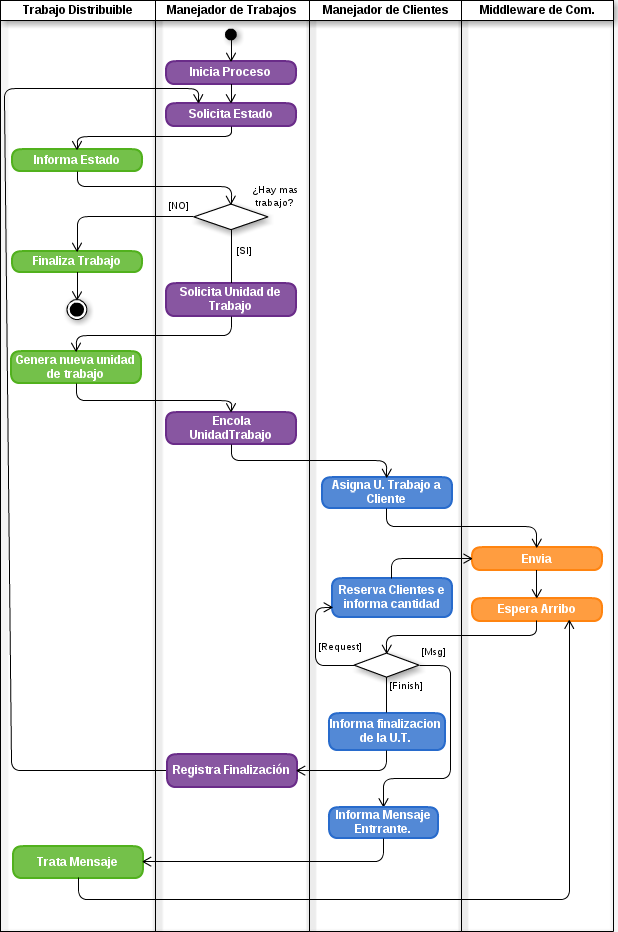
\includegraphics[scale=0.65]{images/ActivityFuDServer-Duplex.png}
    \caption{Diagrama de Actividad de \fud{} refactorizado lado servidor}
    \label{FuDServerDuplex}
\end{figure}

\begin{figure}[ht]
    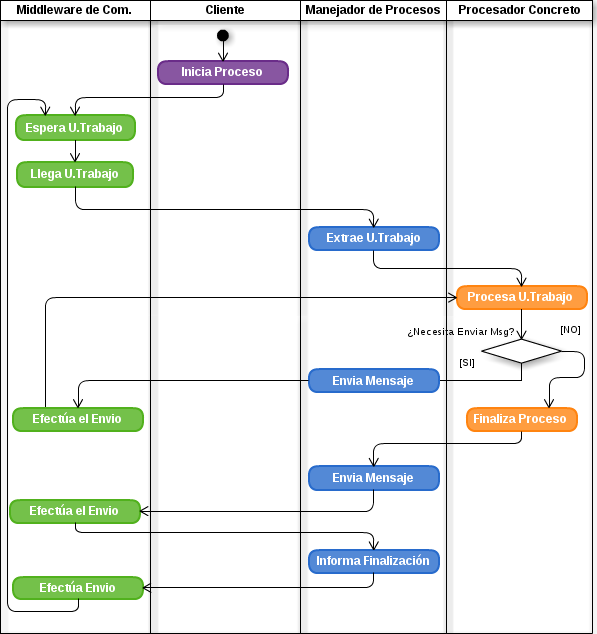
\includegraphics[scale=0.70]{images/ActivityFuDClient-Duplex.png}
    \caption{Diagrama de Actividad de \fud{} refactorizado lado cliente}
    \label{FuDClientDuplex}
\end{figure}

\begin{center}
    \begin{landscape}
        \begin{figure}[ht]
            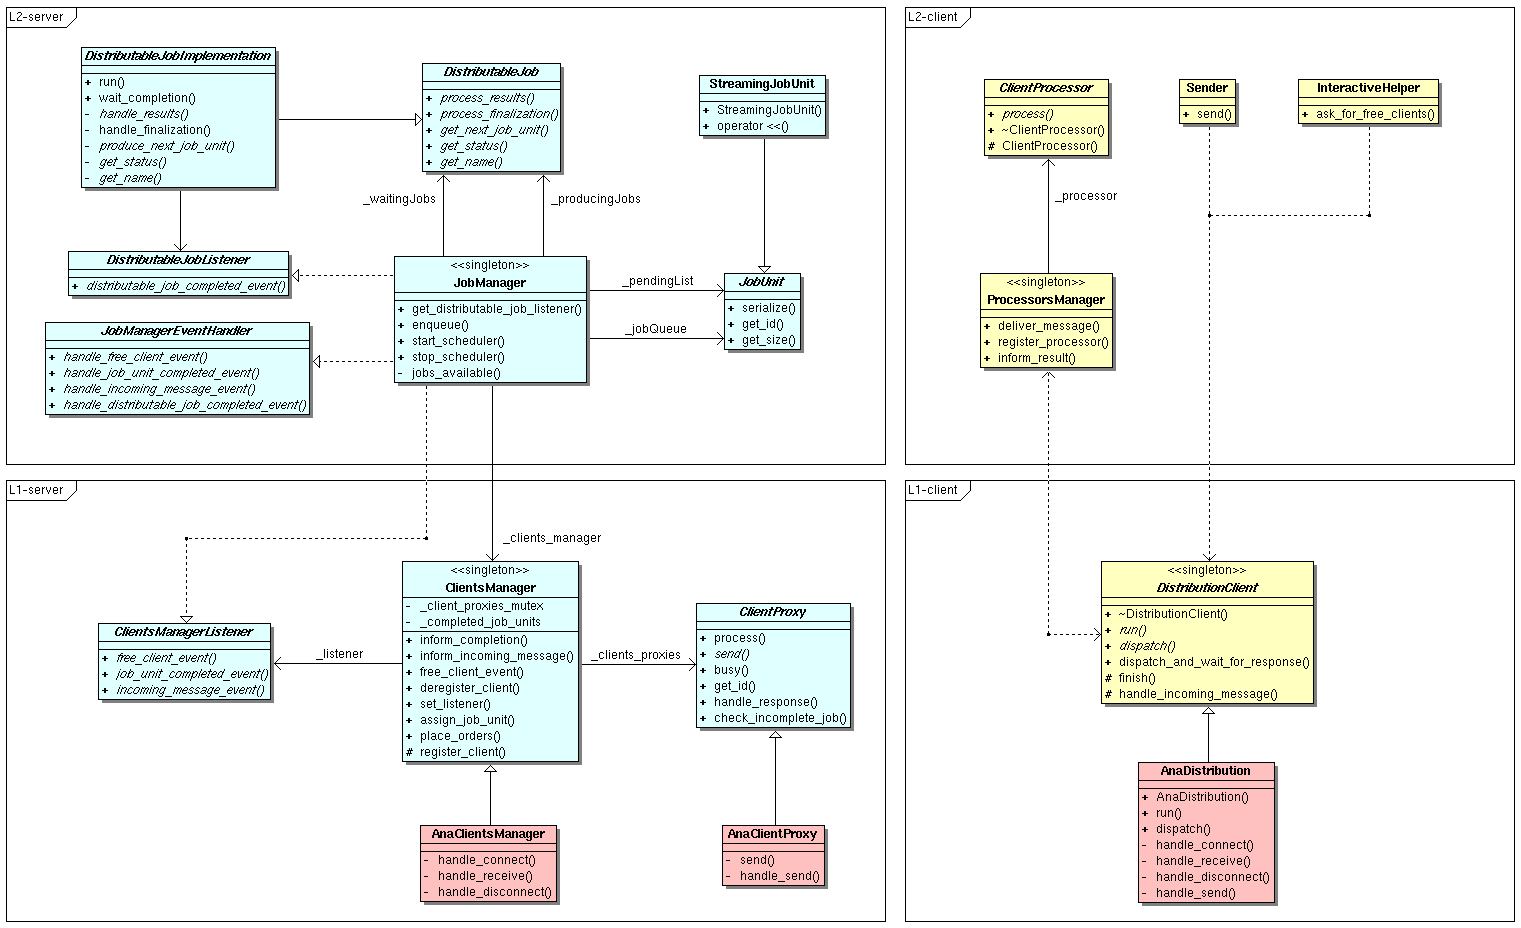
\includegraphics[scale=.38]{images/fud_class.png}
            \caption{Diagrama de clases de \fud{} refactorizado}
            \label{fud_class_diagram}
        \end{figure}
    \end{landscape}
\end{center}


\subsection{Sender}

Se creó esta nueva clase con el simple propósito de servir al cliente con una interfaz para el envío de mensajes. Véase figura
\ref{fud_sender}.

\begin{figure}[ht]
    \begin{center}
        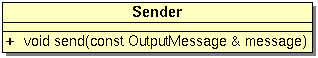
\includegraphics[scale=.75]{images/fud_sender.png}
        \caption{Clase \texttt{Sender}.}
        \label{fud_sender}
    \end{center}
\end{figure}

Este componente tiene una relación directa con la capa L1, encargada de la comunicación con el servidor. El método \texttt{send} adosa, al
mensaje que se desee enviar, un encabezado indicando la presencia de mensaje regular.

\subsection{Ayudante de interactividad}

Este módulo es el encargado de iniciar el pedido y reserva de clientes, por lo que es el artefacto que deben utilizar los clientes de una
aplicación que deseen optar por la reserva de clientes ociosos. Véase figura \ref{fud_interactive_helper}.

\begin{figure}[ht]
    \begin{center}
        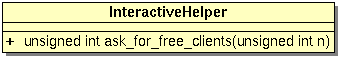
\includegraphics[scale=.75]{images/fud_ihelper.png}
        \caption{Clase \texttt{InteractiveHelper}.}
        \label{fud_interactive_helper}
    \end{center}
\end{figure}

El método \texttt{ask\_for\_free\_clients} toma un número entero, el cuál es el número de clientes deseados por el cliente, luego envía
este requerimiento al servidor, éste calcula, en base al número y la cantidad de clientes ociosos que posee, cuántos clientes le puede
destinar al requeridor. Finalmente, el cliente recibe el número de clientes ociosos que el servidor le pudo asignar. En la figura
\ref{place_orders} se muestra un diagrama de actividad sobre esta interacción de pedido y reserva de clientes.

\begin{figure}[ht]
    \begin{center}
        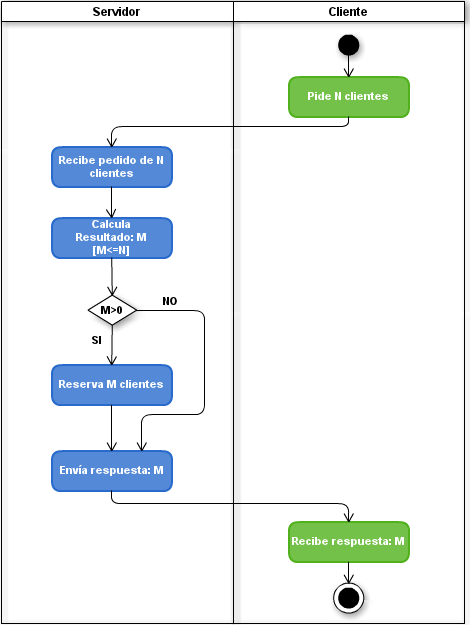
\includegraphics[scale=.65]{images/place_orders.png}
        \caption{Diagrama de actividad de pedido y reserva de clientes}
        \label{place_orders}
    \end{center}
\end{figure}


\section{Implementación}

Como se dijo en la parte de Diseño \ref{redesign_design}, se modificó más de lo que se añadió, por lo que también en lo que respecta a
código, fueron más las líneas aportadas para la adaptación de las nuevas funcionalidades que la implementación de estas nuevas
características en sí.

\subsection{Cambios en \fud}

Aquí hablaremos de los cambios sustanciales que sufrió este software para poder adoptar las nuevas características. Nombraremos las
modificaciones siguiendo la arquitectura cliente/servidor, empezando por los nuevos encabezados de mensaje que se incluyeron, y en cada caso
los servicios que se refactorizaron.

\subsubsection{Servidor}

Los siguientes \textit{headers} corresponden a paquetes enviados de \textbf{clientes al servidor}:
\begin{itemize}
    \item   \texttt{kMessage} : mensaje que será tratado por la aplicación que corra sobre \fud.
    \item   \texttt{kFreeClientsRequest} : usado para pedido y reserva de clientes ociosos.
    \item   \texttt{kJobUnitCompleted} : paquete que informa la finalización de una unidad de trabajo.
\end{itemize}

Cabe destacar que \texttt{kMessage} es el único tipo de mensaje que maneja la aplicación L3, generalmente para resultados y mensajes
intermedios, ambos tratados de la manera que el usuario del framework disponga.

En el caso de un pedido de clientes libres, el servidor cuenta con un \textit{handler} que retorna el número de clientes que dispone para
tal pedido. Para ello, se lleva rastro de todas las reservas hechas de todos los clientes, lo cuál otorga una visión general que permite
obtener el número de clientes realmente disponibles (no reservados) en un momento dado. La respuesta debió ser lo más exacta posible, debido
a que un error en ella se traduce a una ``falsa'' prestación de recursos, y debió ser rápida ya que cuando un cliente realiza esta consulta,
espera una respuesta por parte del servidor sin poder seguir procesando su tarea.

Para incluir el fin de una unidad de trabajo, sólo se tuvo que agregar un nuevo evento que atendiera esta acción. La finalización de un
trabajo puede tener una implementación específica a la aplicación.

\subsubsection{Cliente}

Por otra parte, los mensajes que viajan desde el \textbf{servidor hacia los clientes} pueden ser:
\begin{itemize}
    \item   \texttt{kJob} : representa una unidad de trabajo que ha sido asignada al destinatario.
    \item   \texttt{kFreeClientsResp} : respuesta al pedido de clientes ociosos.
\end{itemize}

El tratamiento de la llegada de una unidad de trabajo esta contemplada en el \fud{} original. La inclusión del manejo a la respuesta del
pedido de clientes trajo aparejada la implementación de una espera bloqueante sobre el cliente, ya que éste no puede seguir procesando su
trabajo pendiente sin una respuesta.


\subsection{Métricas de la refactorización de \fud}

Para analizar el código estáticamente se usaron herramientas como CLOC\footnote{http://cloc.sourceforge.net/} (Count Lines of Code) y
CCCC\footnote{http://cccc.sourceforge.net/} (\textbf{\textit{C}} and \cpp{} Code Counter). En esta sección se describen métricas de
código generales obtenidas por ambas herramientas y se analizan los resultados obtenidos.

El rediseño del framework \fud{} fue realizado con 21 modificaciones de archivos más la creación de otros 5 archivos con un total de 1114
líneas de texto. La tabla \ref{cloc_redesign_fud} resume los resultados obtenidos después de correr CLOC sobre los archivos fuentes.

\begin{table}[!htf]
    \begin{center}
    \begin{tabular}{|l|r|r|r|r|r|c|}
    \hline
    \multicolumn{3}{|c|}{Files} & \multicolumn{3}{|c|}{Line Types} & \hspace{0.2cm}\% \\
    \hline
    \textbf{Type} & \textbf{Mod.} & \textbf{Cre.} & \textbf{Blank} & \textbf{Comment} & \textbf{Source} &
\small{\textbf{Com./Tot.}}\\
    \hline
    \texttt{C++ source} & 9   & 3   &    60  &    176   &   287 & 38.01 \\
    \hline
    \texttt{C++ header} & 12  & 2   &    88  &    403   &   100 & 80.11 \\
    \hline
    \textbf{Total}      & 21  & 5   &   148  &    579   &   387 & 59.93 \\
    \hline
    \end{tabular}
    \caption{Resultados de CLOC para el refactorización de \fud}
    \label{cloc_redesign_fud}
    \end{center}
\end{table}

Haciendo referencia en la sección ``Métricas de \rc''(véase \ref{recabs_metrics}), se dijo que las líneas de código no reflejan la
productividad, más aún que a mayor líneas más complejo es el producto de software, y por lo tanto es más difícil de mantener y comprender.
En lo que respecta a la refactorización de \fud, puede verse que con sólo 387 líneas de código se desarrollaron las nuevas funcionalidades,
que resultaron funcionar como se esperaba.

Como ocurrió en el desarrollo de \rc, existen más líneas de comentario que líneas de código, con una relación de casi 60\%. Esto indica que
se hizo hincapié en la documentación para el mejor entendimiento futuro del funcionamiento del framework. Esta cantidad de comentarios se
deben en gran medida a los encabezados de cada archivo y al uso Doxygen, como ya se explicó en la sección sobre las métricas de \rc.

En el apéndice \ref{fud_metrics_report} se muestra un reporte completo sobre las métricas de código de \fud{} después de su
refactorización, generado con la herramienta CCCC. Incluye muchas métricas de diseño Orientado a Objetos y todo tipo de información
relevante en cuanto a código. Un análisis exhaustivo de los resultados de estas métricas está fuera del alcance de este trabajo. No
obstante, el informe proporciona una visión cuidadosa de la estructura de la librería.
